\documentclass[tikz]{article}
\usepackage[margin=5mm]{geometry}
\usepackage{pgf,tikz}
\usepackage{amsmath}
\usepackage{amssymb}
\usetikzlibrary{shapes,backgrounds,decorations,decorations.pathmorphing}
% Title Page
\title{Title here} 
\author{Dilawar Singh}
\date{\today}
\usetikzlibrary{decorations.text}
\begin{document}
\begin{tikzpicture}[mypostaction/.style 2 args={
        decoration={
            text align={
                left indent=#1},
            text along path, 
            text={#2}
        },
        decorate
    }
    ]

    \edef\lengthScale{16}
    \coordinate (sizeRoot) at (0, 1);
    \coordinate (sizeends) at (0,\lengthScale);
    \coordinate (timeRoot) at (1,0);
    \coordinate (timeends) at (\lengthScale, 0);


    \draw[-latex, blue!20!white, line width=5ex]  (timeRoot) to[] (timeends);
    \draw[-latex, blue!20!white, line width=5ex]  (sizeRoot) to[] (sizeends);


    \node[] (nm) at (0,1) {$10^{-9}m$};
    \node[] (um) at (0,5) {$10^{-6}m$};
    \node[] (mm) at (0,9) {$10^{-3}m$};
    \node[] (m) at (0,13) {$10^{-0}m$};

    \node[] (us) at (1.5,0) {$\mu$ sec};
    \node[] (ms) at (4.5,0) {$m$ sec};
    \node[] (s) at (7.5,0) {sec};
    \node[] (hrs) at (10.5, 0) {hours};
    \node[] (days) at (13.5, 0) {days};

    \node[] (n1) at ([xshift=-1.5cm,yshift=0cm]nm) {
        \includegraphics[width=0.1\textwidth]{../images/8tim_TIM_barrel.png}
    };

    \node[] (n2) at ([xshift=-1.5cm,yshift=0cm]um) {
        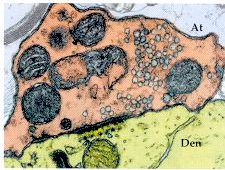
\includegraphics[width=0.1\textwidth]{../images/dendrite.png}
    };

    \node[] (n3) at ([xshift=-1.5cm,yshift=-1cm]mm) {
        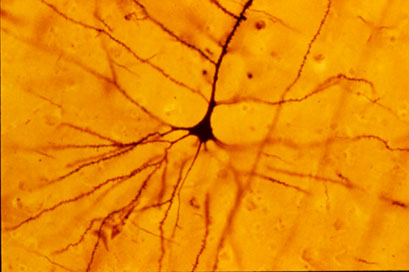
\includegraphics[width=0.1\textwidth]{../images/GolgiStainedPyramidalCell.jpg}
    };

    \node[] (n4) at ([xshift=-1.5cm,yshift=1cm]mm) {
        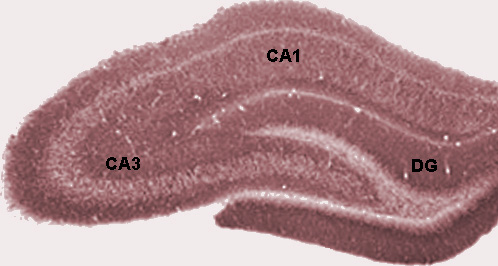
\includegraphics[width=0.1\textwidth]{../images/HippocampalRegions.jpg}
    };

    \node[] (n5) at ([xshift=-1.5cm,yshift=-1.5cm]m) {
        \includegraphics[width=0.1\textwidth]{../images/brain.png}
    };

    \node[rectangle, minimum width=12cm, minimum height=7.0cm,
        fill=blue!10, rounded corners] (chemical) at (9.0,4.5) {};

    \node[] (caption) at ([yshift=-1cm]chemical.north) {\LARGE Chemical};

    \node[rectangle, minimum width=4cm, minimum height=7cm, fill=red!10, rounded corners] 
        (electrical) at (4.0, 11.0) {\LARGE Electrical};

    % Put chemical network here
    \node[] (network) at (7.0,4.0) {
        \includegraphics[width=5cm]{../images/chemical_reactions.png}
    };

    \node[] (chromosome) at (11.0,6.0) {
        
\includegraphics[width=5cm]{../images/chromosome.png}
    };

\end{tikzpicture}

\end{document}

\end{document}          

